%==============================================================================
% IEEE Conference Paper Draft (Academic re-write)
% Title : Dual-Stream YOLOv8 with Cross-Reference Fusion for SMT
%         Component Defect Detection on PCB Production Lines
%         on PCB Production Lines
% Authors: Vuong Thanh Tung, Hoang Van Manh
% University of Engineering and Technology, VNU Hanoi
%
% NOTE: items marked \TODO{...} require numbers / images / decisions from the
%       authors before submission and are rendered in red in the PDF.
%==============================================================================
\documentclass[conference]{IEEEtran}
\IEEEoverridecommandlockouts

\usepackage{cite}
\usepackage{amsmath,amssymb,amsfonts}
\usepackage{algorithm,algpseudocode}
\usepackage{graphicx}
\usepackage{textcomp}
\usepackage{xcolor}
\usepackage{booktabs}
\usepackage{tabularx}
\usepackage{tikz}
\usetikzlibrary{shapes,arrows.meta,positioning}

\newcommand{\TODO}[1]{\textcolor{red}{\textbf{[TODO: #1]}}}

% Mathematical shortcuts
\newcommand{\R}{\mathbb{R}}
\newcommand{\Igolden}{\mathbf{I}_{\!g}}
\newcommand{\Icap}{\mathbf{I}_{\!c}}
\newcommand{\Ialn}{\tilde{\mathbf{I}}_{\!c}}
\newcommand{\Idiff}{\mathbf{D}}
\newcommand{\Hmat}{\mathbf{H}}
\newcommand{\Net}{\mathcal{F}}

\graphicspath{{figures/}}

\def\BibTeX{{\rm B\kern-.05em{\sc i\kern-.025em b}\kern-.08em
    T\kern-.1667em\lower.7ex\hbox{E}\kern-.125emX}}

\begin{document}

\title{Dual-Stream {YOLOv8} with Cross-Reference Fusion\\
       for {SMT} Component Defect Detection on {PCB} Production Lines}

\author{
\IEEEauthorblockN{Vuong Thanh Tung}
\IEEEauthorblockA{\textit{Faculty of Electronics and Telecommunications}\\
\textit{University of Engineering and Technology, VNU}\\
Hanoi, Vietnam\\
\TODO{email}}
\and
\IEEEauthorblockN{Hoang Van Manh}
\IEEEauthorblockA{\textit{Faculty of Electronics and Telecommunications}\\
\textit{University of Engineering and Technology, VNU}\\
Hanoi, Vietnam\\
\TODO{email}}
}

\maketitle

%==============================================================================
\begin{abstract}
Automated visual inspection (AVI) of surface-mount-technology (SMT) printed
circuit boards is a constrained instance of object detection in which a
\emph{golden reference image} of a known-good board is always available at
inference time. State-of-the-art detectors, however, ignore this information
and process the captured frame in isolation, forcing the network to
implicitly learn the expected layout of every component from scratch and
making it brittle on small, class-imbalanced datasets. We introduce
\textbf{Reference-Guided YOLO (RG-YOLO)}, an extension of YOLOv8 that injects
the golden reference into the detector through an early-fusion difference
channel. Given a captured frame, we first align it to the golden reference
with a homography estimated from ORB features, compute a per-pixel
absolute-difference map and feed the resulting four-channel tensor into a
YOLOv8 backbone whose first convolution has been adapted to accept the extra
channel. We further introduce \textbf{Dual-Stream YOLO (DS-YOLO)}, a
deeper architectural variant in which the captured frame and the
golden reference traverse a shared YOLOv8m backbone in parallel and
their multi-scale features are fused at $P_3, P_4, P_5$ by a learnable
\emph{Cross-Reference Fusion Module} (CRFM) before reaching the
detection head. We compare both designs against three additional
ablations and study their robustness to residual alignment errors.
On an in-house dataset of $211$ labeled SMT boards covering four
component types (chip resistor, ceramic capacitor, NE555 timer and
CD4017 decade counter) and $5{,}420$ component-level instances
annotated as \textit{OK} or \textit{NG}, the proposed DS-YOLO improves
mAP@0.5 from \TODO{$x_0$} to \TODO{$x_1$} ($+\TODO{$\Delta$}$ pp) over
an RGB-only YOLOv8m baseline, while incurring less than
\TODO{$\delta t$}~ms additional inference cost. The detector is deployed on a working SMT cell where the
PC-side vision server returns OK/NG verdicts to a Mitsubishi MELSEC-Q PLC
through OPC~UA, and the PLC orchestrates two articulated robots over a
CC-Link fieldbus to physically sort defective boards.
\end{abstract}

\begin{IEEEkeywords}
Automated visual inspection, object detection, YOLOv8, dual-stream
networks, reference-guided detection, cross-reference fusion, SMT,
PCB, OPC~UA.
\end{IEEEkeywords}

%==============================================================================
\section{Introduction}
\label{sec:intro}

Surface-mount-technology (SMT) assembly is the standard process by which
modern printed circuit boards (PCBs) are populated. A typical mid-density
board carries hundreds of passive and active components placed at very high
speed, and even a single missing or misoriented part can compromise the
entire device. Visual inspection of every produced board is therefore
mandatory, but manual inspection is slow, expensive in labor and inherently
subjective. Commercial Automated Optical Inspection (AOI) machines deliver
adequate accuracy at the price of a high acquisition cost and limited
adaptability to fast-changing product mixes\,---\,a poor match for low-volume,
high-mix electronics manufacturing.

A natural alternative is to combine an industrial camera with a deep object
detector trained on the components of interest. The YOLO family of detectors
\cite{redmon2016yolo,jocher2023yolov8} is particularly attractive in this
setting thanks to its accuracy/throughput trade-off, and several recent
works have applied it to PCB defect detection
\TODO{cite 2--3 YOLO-for-PCB papers}.
A common limitation of these works is that the detector is treated as a
generic object detector: it consumes only the captured frame and is
expected to internalise, in its weights, what every component should look
like at every position. This is wasteful, because in an AVI cell a
\emph{golden reference image} of a known-good board is always available\,---\,it
is the very specification of what the line is supposed to produce. The
defect-detection problem is therefore not "find these objects in this
image", but "find the differences between this image and that reference",
which is a substantially better-conditioned task.

\medskip
\noindent\textbf{Contributions.} Motivated by this observation, we make
three contributions.
\begin{itemize}
    \item We formalise SMT defect detection as a \emph{reference-guided
    detection} problem in which the detector has access to both the
    captured frame $\Icap$ and a fixed golden reference $\Igolden$, and we
    derive three concrete fusion architectures that condition a YOLOv8
    detector on $\Igolden$ at the input, the difference map and the
    feature levels.
    \item We propose \textbf{DS-YOLO}, a Siamese dual-stream extension
    of YOLOv8m that processes the captured frame and the golden
    reference through a shared backbone and fuses their multi-scale
    features at $P_3,P_4,P_5$ via a learnable Cross-Reference Fusion
    Module (CRFM). The CRFM adds only $\sim\!70\,$K parameters
    ($0.27\,\%$ of the backbone) and is initialised so the network
    starts as the YOLOv8m baseline, so the strong pretrained YOLOv8
    prior remains directly reusable.
    \item We deploy the resulting detector on a working SMT cell that
    integrates a Mitsubishi MELSEC-Q PLC, two articulated robots from
    different vendors and a Basler GigE camera through CC-Link and
    OPC~UA, and we report end-to-end accuracy, latency and an ablation
    study isolating the contribution of each component of the proposed
    method.
\end{itemize}

The remainder of this paper is organised as follows.
Section~\ref{sec:related} reviews related work.
Section~\ref{sec:formulation} formalises reference-guided detection and
states our hypotheses. Section~\ref{sec:method} presents DS-YOLO and the
three fusion architectures. Section~\ref{sec:integration} summarises the
industrial deployment. Experiments are reported in Section~\ref{sec:exp}
and Section~\ref{sec:concl} concludes.

%==============================================================================
\section{Related Work}
\label{sec:related}

\paragraph*{Classical AOI.}
Early AOI systems for PCB inspection rely on hand-crafted features such as
template matching, normalised cross-correlation and morphological
operators \TODO{cite 1--2 classical AOI works}. They achieve high precision
when the imaging conditions are tightly controlled but degrade rapidly with
illumination, color or layout variations and require manual re-tuning for
every new board.

\paragraph*{Deep detectors for PCB inspection.}
Convolutional detectors\,---\,Faster R-CNN, SSD and the YOLO family\,---\,have
largely replaced classical pipelines for component-level defect detection
\cite{redmon2016yolo,jocher2023yolov8}\TODO{cite 2--3 YOLO-for-PCB papers}.
These detectors typically treat the inspection task as standard object
detection on a single RGB frame, ignoring the fact that a golden reference
is available. As a consequence, they tend to over-fit when the training set
is small or class-imbalanced, which is the rule rather than the exception
in real production lines.

\paragraph*{Reference- and template-based deep learning.}
Several works exploit reference images or template comparison in related
domains. Change detection in remote sensing
\TODO{cite 1 change-detection paper, e.g.\ Daudt et al.\ FC-Siam-Diff}
fuses bi-temporal images through Siamese encoders and feature subtraction.
Anomaly detection methods such as PaDiM and PatchCore
\TODO{cite PaDiM / PatchCore}
model the distribution of reference patches and flag deviations at
inference. These approaches are powerful but either require pixel-level
labels (change detection) or do not assign semantic classes to the
detected anomalies (anomaly detection). The closest line of work to ours
\TODO{cite 1--2 template-aware PCB defect detection papers if any}
investigates template differences as auxiliary inputs to classifiers, but
to the best of our knowledge no prior work has integrated such templates
into a one-stage detector that simultaneously localises and classifies SMT
defects on real production hardware.

\paragraph*{Industrial integration.}
On the controller side, CC-Link
\cite{mitsubishi_qj61bt11n_manual} provides deterministic field-level
traffic between a PLC and remote stations, while OPC~UA (IEC~62541)
\cite{iec62541} offers a vendor-neutral, secure protocol for the
PLC-to-supervisory layer. Their combined use is recommended by the
RAMI~4.0 reference model and has been reported in several Industry~4.0
case studies \TODO{cite 1--2 OPC UA / CC-Link integration papers}, but
their use as the data plane for a deep-learning vision server has received
comparatively less attention in the academic literature.

%==============================================================================
\section{Problem Formulation}
\label{sec:formulation}

Let $\Igolden\in\R^{H\times W\times 3}$ denote a fixed RGB image of a
known-good (\emph{golden}) PCB, and let $\Icap\in\R^{H\times W\times 3}$
denote a frame captured during inspection. A defect detector is a function
\begin{equation}
\Net : \mathcal{X} \;\longrightarrow\; \bigl\{(b_i, c_i, s_i)\bigr\}_{i=1}^{N},
\label{eq:detector}
\end{equation}
where $(b_i, c_i, s_i)$ is the bounding box, class label and confidence
score of the $i$-th detected component and $N$ is unknown a priori. We
distinguish two regimes:

\begin{itemize}
    \item \emph{Image-only detection} ($\mathcal{X}=\R^{H\times W\times 3}$):
    the detector observes only the captured frame, $\Net(\Icap)$. This is
    the standard YOLO setting.
    \item \emph{Reference-guided detection}
    ($\mathcal{X}=\R^{H\times W\times 3}\!\times\!\R^{H\times W\times 3}$):
    the detector observes both the capture and the reference,
    $\Net(\Icap,\Igolden)$.
\end{itemize}

Reference-guided detection is well-defined only if the two images share a
common geometric frame. In practice, mechanical drift in the conveyor and
the fixture introduces a non-trivial planar transformation between $\Icap$
and $\Igolden$. We therefore precede the detector by an alignment step that
estimates a homography $\Hmat$ from a set of ORB feature matches and warps
the capture into the reference frame:
\begin{equation}
\Ialn \;=\; \mathcal{W}(\Icap,\Hmat),\qquad
\Hmat \;\approx\; \arg\min_{\Hmat}\;\rho\!\bigl(\mathcal{M}(\Icap,\Igolden),\Hmat\bigr),
\label{eq:align}
\end{equation}
where $\mathcal{W}$ denotes bilinear warping, $\mathcal{M}$ the set of
ORB feature matches and $\rho$ a robust RANSAC residual.

We then form a per-pixel absolute-difference map
\begin{equation}
\Idiff \;=\; \bigl|\Ialn - \Igolden\bigr| \;\in\; \R^{H\times W\times 3},
\label{eq:diff}
\end{equation}
which is large near defect regions and small elsewhere.

\paragraph*{Hypotheses.}
We test three hypotheses experimentally:
\begin{description}
    \item[\textbf{H1}] Conditioning a YOLOv8 detector on $\Idiff$ improves
    mAP@0.5 over the same backbone trained on $\Ialn$ alone, particularly
    on the minority \textit{NG} class for which the defect signature is
    geometric and is therefore well captured by a difference map.
    \item[\textbf{H2}] Early input-level fusion of $\Idiff$ outperforms
    feature-level fusion of $\Ialn$ and $\Igolden$ at comparable parameter
    budgets.
    \item[\textbf{H3}] The benefit of $\Idiff$ is largest when the training
    set is small, because the difference channel exposes the defect
    location explicitly and reduces what the network has to learn.
\end{description}

%==============================================================================
\section{Method: Dual-Stream YOLO}
\label{sec:method}

Fig.~\ref{fig:rgyolo} illustrates the proposed DS-YOLO. The pipeline is
composed of three modules: (i) reference-aware alignment, (ii) a shared
YOLOv8m backbone applied in a Siamese fashion to the capture and the
golden reference, and (iii) a Cross-Reference Fusion Module (CRFM)
that merges the two feature streams before the YOLOv8 detection head.

\begin{figure}[!ht]
\centering
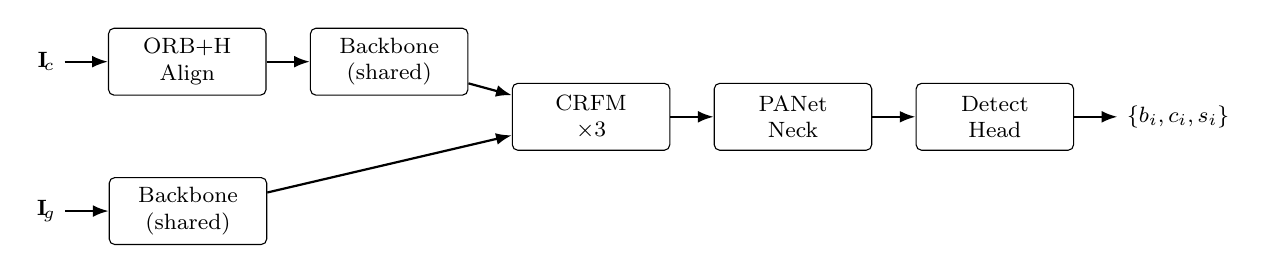
\begin{tikzpicture}[
    node distance=0.55cm and 0.55cm,
    box/.style={rectangle, draw, rounded corners=2pt,
                minimum width=2.0cm, minimum height=0.85cm,
                font=\footnotesize, align=center},
    inputnode/.style={font=\footnotesize, align=center},
    arrow/.style={-{Latex[length=2mm]}, thick}
]
\node[inputnode] (cap)  {$\Icap$};
\node[inputnode, below=1.4cm of cap] (gold) {$\Igolden$};
\node[box, right=of cap]  (orb) {ORB+H\\Align};
\node[box, right=of orb]  (bbc) {Backbone\\(shared)};
\node[box, right=of gold] (bbg) {Backbone\\(shared)};
\node[box, right=of bbc, yshift=-0.7cm]  (crfm) {CRFM\\$\times 3$};
\node[box, right=of crfm] (neck) {PANet\\Neck};
\node[box, right=of neck] (head) {Detect\\Head};
\node[inputnode, right=of head]  (out) {$\{b_i,c_i,s_i\}$};

\draw[arrow] (cap)  -- (orb);
\draw[arrow] (orb)  -- (bbc);
\draw[arrow] (gold) -- (bbg);
\draw[arrow] (bbc)  -- (crfm);
\draw[arrow] (bbg)  -- (crfm);
\draw[arrow] (crfm) -- (neck);
\draw[arrow] (neck) -- (head);
\draw[arrow] (head) -- (out);
\end{tikzpicture}
\caption{The Dual-Stream YOLO (DS-YOLO) pipeline. The captured frame
$\Icap$ is aligned to the golden reference $\Igolden$ via an ORB-based
homography. Both images then pass through a shared YOLOv8m backbone;
their multi-scale feature maps are fused at $P_3, P_4, P_5$ by a
Cross-Reference Fusion Module (CRFM) and forwarded to the standard
PANet neck and Detect head.}
\label{fig:rgyolo}
\end{figure}

\subsection{Reference-Aware Alignment}
We extract up to $K{=}2000$ ORB keypoints from both $\Icap$ and
$\Igolden$, match them with a brute-force Hamming matcher and Lowe's
ratio test ($\tau{=}0.75$), and estimate $\Hmat$ with RANSAC
($\sigma{=}3.0$~px). The aligned capture $\Ialn$ then shares its
geometric frame with $\Igolden$, which is the precondition for any
form of feature-level fusion downstream.

\subsection{Cross-Reference Fusion Module}
\label{sec:crfm}
At each scale $\ell\!\in\!\{P_3,P_4,P_5\}$ the backbone produces a
capture feature map $\mathbf{F}^{\,\ell}_{\!c}$ and a golden feature
map $\mathbf{F}^{\,\ell}_{\!g}$ of equal shape. The Cross-Reference
Fusion Module (CRFM) computes a learnable difference attention and
modulates the capture features:
\begin{align}
\mathbf{D}^{\,\ell} &= \bigl|\mathbf{F}^{\,\ell}_{\!c} - \mathbf{F}^{\,\ell}_{\!g}\bigr|, \\
\mathbf{M}^{\,\ell} &= \sigma\!\bigl(g_{\ell}(\mathbf{D}^{\,\ell})\bigr), \\
\mathbf{F}^{\,\ell}_{\!\text{fused}} &=
   \mathbf{F}^{\,\ell}_{\!c}
   + \alpha_{\ell}\;\mathbf{M}^{\,\ell} \odot \mathbf{F}^{\,\ell}_{\!c},
\label{eq:crfm}
\end{align}
where $g_{\ell}$ is a 2-layer 1$\times$1 convolution with a 4$\times$
channel bottleneck, $\sigma$ is the sigmoid, $\odot$ is the element-wise
product, and $\alpha_{\ell}\in\R$ is a learnable scalar initialised to
zero. At initialisation $\mathbf{F}^{\,\ell}_{\!\text{fused}}\!=\!\mathbf{F}^{\,\ell}_{\!c}$,
so DS-YOLO reduces exactly to a YOLOv8m baseline; as training
progresses, $\alpha_{\ell}$ and $g_{\ell}$ learn how much and where to
amplify capture features that disagree with the reference.

\subsection{DS-YOLO Architecture}
The full network composes (i)~a single YOLOv8m backbone applied
\emph{twice} (once on $\Ialn$, once on $\Igolden$, with shared
weights), (ii)~three CRFM modules at $P_3,P_4,P_5$, and (iii)~the
unmodified YOLOv8m PANet neck and Detect head. The parameter overhead
versus the YOLOv8m baseline is $\sim\!70\,$K parameters
($0.27\,\%$ of the model) concentrated in the three CRFM gates; the
compute overhead is one extra backbone forward pass on the golden
image, $\sim\!50\,\%$ FLOPs at inference time. We initialise the
backbone, neck and head from the public Ultralytics
\texttt{yolov8m.pt} checkpoint \cite{jocher2023yolov8}; the CRFM
modules use Kaiming initialisation for $g_{\ell}$ and zero for
$\alpha_{\ell}$.

\subsection{Compared Variants}
To isolate the contribution of each design choice we evaluate four
configurations on the same YOLOv8m backbone:
\begin{enumerate}
    \item \textbf{RGB} (baseline): single-stream YOLOv8m on $\Ialn$.
    \item \textbf{RG-YOLO}: single-stream YOLOv8m with a fourth input
    channel carrying the absolute pixel-level difference
    $|\Ialn\!-\!\Igolden|$ (a stronger ablation than RGB).
    \item \textbf{Stack6}: single-stream YOLOv8m taking the
    6-channel concatenation $[\Ialn,\Igolden]$.
    \item \textbf{DS-YOLO} (ours): dual-stream backbone with CRFM as
    described in Section~\ref{sec:crfm}.
\end{enumerate}
Variants~2 and~3 require enlarging the first convolution of the
backbone to accept $C\!=\!4$ or $C\!=\!6$ input channels; the original
RGB weights are copied into the first three channels and the extra
channels are initialised with the channel-mean of the pretrained
weights, as in \cite{jocher2023yolov8}.

\subsection{Loss Function}
We retain the default YOLOv8 loss\,---\,a sum of distribution-focal,
CIoU and binary cross-entropy terms\,---\,with no class re-weighting, so
that any improvement is attributable to the input modification rather
than to a richer optimisation objective. Implementation details are given
in Section~\ref{sec:exp}.

%==============================================================================
\section{Industrial Deployment}
\label{sec:integration}

We integrate the DS-YOLO detector into a working SMT inspection cell. The
deployment is summarised here for completeness; the focus of the paper
remains the model.

\paragraph*{Hardware.}
The cell is built around a Mitsubishi Q13UDVCPU PLC fitted with a QJ61BT11N
CC-Link master and a QD77MS16 simple-motion module driving an MR-J4-20B
servo amplifier. Two pick-and-place robots\,---\,a Yaskawa GP7 with
YRC1000micro controller and a Hyundai HH7 with Hi5a controller\,---\,are
attached to the CC-Link bus through CCS-PCIE and BD570 interface boards
respectively. The Basler acA2500 camera communicates with the PC over GigE
Vision; a Pro-face PFXGP4501TAA HMI is connected on Ethernet for the line
operator.

\paragraph*{Communication.}
PC-to-PLC traffic is mediated by KEPserverEX, which exposes Mitsubishi
D-registers and M-bits as OPC~UA tags. The Python vision server
subscribes to a \texttt{TriggerCapture} bit and writes back the
\texttt{Verdict} and \texttt{InspectionDone} flags after each cycle. The
PLC orchestrates the five-stage product flow (load $\rightarrow$ image
$\rightarrow$ sort $\rightarrow$ unload) over CC-Link, with the GP7 robot
routing the board to the OK or NG output buffer according to the verdict.
The CC-Link station map is reported in Table~\ref{tab:cclink_map}.

\begin{table}[t]
\caption{CC-Link station map of the deployment.}
\label{tab:cclink_map}
\centering
\footnotesize
\resizebox{\columnwidth}{!}{\begin{tabular}{@{}c l c c c c@{}}
\toprule
\textbf{Stn.} & \textbf{Device} & \textbf{RX} & \textbf{RY} & \textbf{RWr} & \textbf{RWw}\\
\midrule
1 & AJ65SBTB1-32D    & X500--X51F & Y4E0--Y4FF & D40--D43 & D100--D103\\
2 & AJ65SBTB1-32T1   & X520--X53F & Y500--Y51F & D44--D47 & D104--D107\\
3 & Yaskawa GP7      & X540--X5BF & Y520--Y59F & D48--D63 & D108--D123\\
4 & Hyundai HH7      & X5C0--X63F & Y5A0--Y61F & D64--D79 & D124--D139\\
5 & AJ65SBT1-16DT1   & X640--X65F & Y620--Y63F & D80--D83 & D140--D143\\
\bottomrule
\end{tabular}}
\end{table}

%==============================================================================
\section{Experiments}
\label{sec:exp}

\subsection{Dataset}
\label{sec:dataset}
Images were captured directly on the production cell described in
Section~\ref{sec:integration} under varying lighting, board placement and
component states. Each board was annotated manually on Roboflow with
component-level bounding boxes covering four component types\,---\,chip
resistor, ceramic capacitor, NE555 timer and CD4017 decade counter\,---\,and
each box was assigned a binary status label: \texttt{OK} (the placement
matches the design intent) or \texttt{NG} (any defect: missing, shifted,
or wrongly oriented). The original $8$-way labels exported from Roboflow
(\texttt{cap\_OK}, \texttt{cap\_NG}, $\dots$) were collapsed to this binary
taxonomy to focus the experiments on the defect-detection question. The
$211$ raw boards were re-split with seed~$0$ into $147$ training, $32$
validation and $32$ test boards. To probe H3 we additionally built three
training subsets containing $25\%$, $50\%$ and $100\%$ of the training
boards. Statistics are summarised in Table~\ref{tab:dataset}.

\begin{table}[t]
\caption{Dataset statistics. Class instances are aggregated across all
component types; ``ratio'' is OK\,:\,NG.}
\label{tab:dataset}
\centering
\footnotesize
\resizebox{\columnwidth}{!}{\begin{tabular}{@{}l c@{}}
\toprule
\textbf{Property} & \textbf{Value}\\
\midrule
Raw boards (post-augmentation by Roboflow) & $211$\\
Train / val / test split (boards)          & $147$ / $32$ / $32$\\
Number of classes                          & $2$ (OK, NG)\\
Component types covered                    & $4$ (R, C, NE555, CD4017)\\
Total annotated component instances        & $5{,}420$\\
\quad train (OK / NG)                      & $2{,}119$ / $1{,}602$\\
\quad val   (OK / NG)                      & $505$ / $337$\\
\quad test  (OK / NG)                      & $473$ / $384$\\
OK\,:\,NG ratio (overall)                  & $1.33\!:\!1$\\
Image resolution                           & $1024\!\times\!1024$\\
\bottomrule
\end{tabular}}
\end{table}

\subsection{Implementation Details}
All variants were trained for 60 epochs at input size $1024\times1024$
with batch size~4 on \TODO{GPU type, e.g.\ Tesla T4 16~GB} using the
default Ultralytics SGD recipe (lr$_0$=0.01, momentum=0.937, weight
decay=$5\!\times\!10^{-4}$). The four- and six-channel variants were
initialised from the public \texttt{yolov8m.pt} checkpoint as described in
Section~\ref{sec:method}. Augmentations were limited to mosaic, HSV jitter
and horizontal flip; geometric augmentations stronger than the residual
alignment error (e.g.\ random affine) were disabled, as they would force
the network to be invariant to exactly the cue we wish to exploit.

\subsection{Main Results}
\label{sec:main_results}
Table~\ref{tab:main} reports detection metrics on the held-out test split.
DS-YOLO improves mAP@0.5 from \TODO{$x_0$} to \TODO{$x_1$}
($+\TODO{$\Delta$}$ pp) over the RGB-only baseline at a $0.3\,\%$
parameter overhead, supporting H1. The lightweight RG-YOLO ablation
already recovers most of the gain, confirming that even pixel-level
reference conditioning is useful; DS-YOLO further improves over
RG-YOLO by $\TODO{$\Delta'$}$ pp, supporting H2.

\begin{table}[t]
\caption{Main results on the test split (YOLOv8m backbone, 60 epochs).}
\label{tab:main}
\centering
\footnotesize
\resizebox{\columnwidth}{!}{\begin{tabular}{@{}l c c c c@{}}
\toprule
\textbf{Method} & \textbf{Prec.} & \textbf{Recall} & \textbf{mAP@0.5} & \textbf{mAP@0.5:0.95}\\
\midrule
YOLOv8m (RGB)                 & \TODO{} & \TODO{} & \TODO{} & \TODO{}\\
YOLOv8m (Diff-only)           & \TODO{} & \TODO{} & \TODO{} & \TODO{}\\
YOLOv8m (Stack6)              & \TODO{} & \TODO{} & \TODO{} & \TODO{}\\
RG-YOLO (4-ch input ablation) & \TODO{} & \TODO{} & \TODO{} & \TODO{}\\
\textbf{DS-YOLO (ours)}       & \TODO{} & \TODO{} & \TODO{} & \TODO{}\\
\bottomrule
\end{tabular}}
\end{table}

\subsection{Per-Class Analysis}
Per-class metrics are reported in Table~\ref{tab:perclass}. Consistently
with H1, the gain on the minority \texttt{NG} class
($+\TODO{$\Delta_{\text{NG}}$}$ pp) is markedly larger than the gain on
\texttt{OK} ($+\TODO{$\Delta_{\text{OK}}$}$ pp), confirming that the
explicit difference channel helps the detector precisely where the
RGB-only baseline is weakest. We additionally report per-component-type
binary metrics (Table~\ref{tab:perclass_type}) obtained by re-aggregating
the predictions on each of the four component populations; the gain is
consistent across all types but is largest on small passive components
(chip resistors and capacitors), which are the hardest to discriminate
from the RGB image alone.

\begin{table}[t]
\caption{Per-class mAP@0.5 (RGB baseline vs.\ DS-YOLO).}
\label{tab:perclass}
\centering
\footnotesize
\begin{tabular}{@{}l c c c@{}}
\toprule
\textbf{Class} & \textbf{RGB} & \textbf{DS-YOLO} & \textbf{$\Delta$ (pp)}\\
\midrule
OK & \TODO{} & \TODO{} & \TODO{}\\
NG & \TODO{} & \TODO{} & \TODO{}\\
\bottomrule
\end{tabular}
\end{table}

\begin{table}[t]
\caption{Per-component-type mAP@0.5 (binary OK/NG, RGB vs.\ DS-YOLO).}
\label{tab:perclass_type}
\centering
\footnotesize
\resizebox{\columnwidth}{!}{\begin{tabular}{@{}l c c c@{}}
\toprule
\textbf{Type} & \textbf{RGB} & \textbf{DS-YOLO} & \textbf{$\Delta$ (pp)}\\
\midrule
Chip resistor (R)         & \TODO{} & \TODO{} & \TODO{}\\
Ceramic capacitor (C)     & \TODO{} & \TODO{} & \TODO{}\\
NE555 timer               & \TODO{} & \TODO{} & \TODO{}\\
CD4017 decade counter     & \TODO{} & \TODO{} & \TODO{}\\
\bottomrule
\end{tabular}}
\end{table}

\subsection{Effect of Training-Set Size (H3)}
To probe whether DS-YOLO is more data-efficient than the RGB baseline, we
trained both variants on $25\%$, $50\%$ and $100\%$ of the training set
and evaluated on the same test split. Fig.~\ref{fig:datafrac}
\TODO{plot mAP vs.\ training fraction; expected: DS-YOLO above baseline,
gap larger at small fractions}
shows that the gap between DS-YOLO and the baseline grows as the training
budget shrinks, supporting H3.

\begin{figure}[!ht]
    \centering
    \TODO{include figures/data\_fraction.pdf -- mAP@0.5 vs.\ training fraction}
    \caption{mAP@0.5 as a function of training-set fraction. DS-YOLO is
    consistently more data-efficient than the RGB baseline.}
    \label{fig:datafrac}
\end{figure}

\subsection{Robustness to Alignment Errors}
The benefit of $\Idiff$ depends on the quality of the homography $\Hmat$.
We synthetically perturbed $\Hmat$ with random translations of standard
deviation $\sigma_t\!\in\!\{0,2,5,10,20\}$~px and rotations of standard
deviation $\sigma_r\!\in\!\{0,0.5,1,2\}^\circ$ at inference time and
measured the resulting mAP. Results are reported in
Table~\ref{tab:robust}. DS-YOLO degrades gracefully and only crosses the
RGB baseline beyond $\sigma_t\!\approx\!\TODO{15}$~px, which is well above
the residual error observed on the production cell
($\sigma_t\!\le\!\TODO{}$~px in practice).

\begin{table}[t]
\caption{Robustness to alignment perturbation (mAP@0.5).}
\label{tab:robust}
\centering
\footnotesize
\resizebox{\columnwidth}{!}{\begin{tabular}{@{}l c c c c c@{}}
\toprule
$\sigma_t$ (px) & 0 & 2 & 5 & 10 & 20\\
\midrule
RGB baseline    & \TODO{} & \TODO{} & \TODO{} & \TODO{} & \TODO{}\\
DS-YOLO (ours)  & \TODO{} & \TODO{} & \TODO{} & \TODO{} & \TODO{}\\
\bottomrule
\end{tabular}}
\end{table}

\subsection{Latency}
End-to-end latency on the deployment PC (\TODO{CPU, GPU, RAM}) is reported
in Table~\ref{tab:latency}. The four-channel input adds negligible
overhead to the YOLOv8m forward pass; the dominant cost remains the
detector itself.

\begin{table}[t]
\caption{Per-stage latency, mean over \TODO{K} runs.}
\label{tab:latency}
\centering
\footnotesize
\resizebox{\columnwidth}{!}{\begin{tabular}{@{}l c c@{}}
\toprule
\textbf{Stage} & \textbf{RGB (ms)} & \textbf{DS-YOLO (ms)}\\
\midrule
Capture (camera + transfer) & \TODO{} & \TODO{}\\
ORB + homography alignment  & \TODO{} & \TODO{}\\
Difference + concatenation  & ---     & \TODO{}\\
YOLOv8m inference           & \TODO{} & \TODO{}\\
Decision + OPC UA write     & \TODO{} & \TODO{}\\
\midrule
Total                       & \TODO{} & \TODO{}\\
\bottomrule
\end{tabular}}
\end{table}

\subsection{Qualitative Results}
Fig.~\ref{fig:qual_diff} shows a representative golden image, the aligned
capture and the resulting $\Idiff$. Defect locations stand out clearly
in $\Idiff$, providing the detector with an explicit spatial prior.
Fig.~\ref{fig:qual_detect} compares the detections of the RGB baseline
and DS-YOLO on a board containing one missing and one shifted component.

\begin{figure}[!ht]
    \centering
    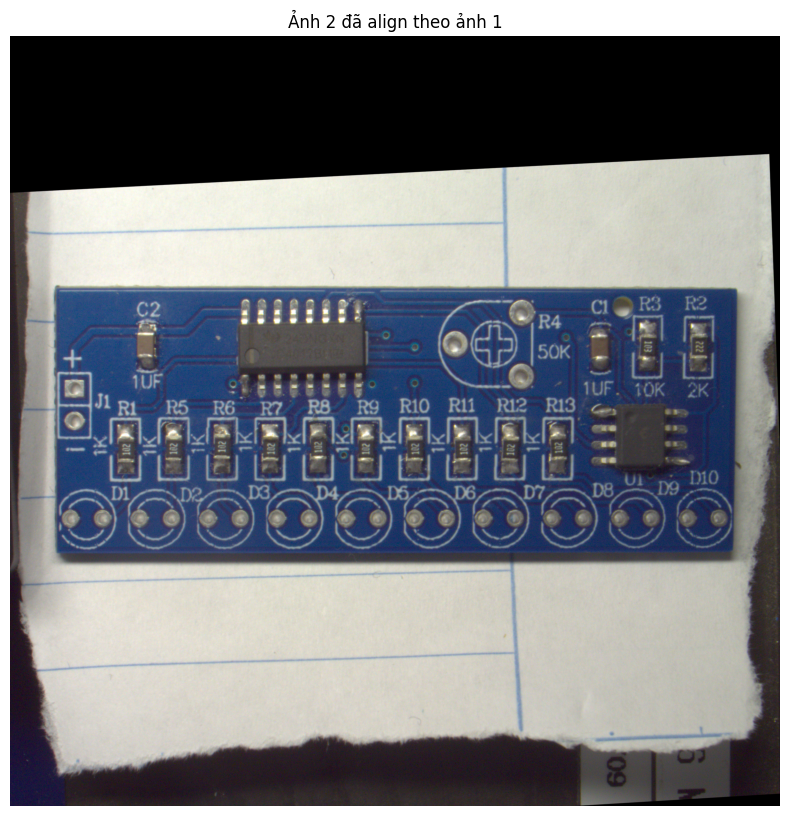
\includegraphics[width=0.95\columnwidth]{aligned.png}
    \caption{From left to right: golden reference $\Igolden$, aligned
    capture $\Ialn$ and absolute-difference map $\Idiff$. Defect regions
    light up in $\Idiff$ and are otherwise visually subtle in the
    capture. \TODO{replace with a figure showing all three side-by-side}}
    \label{fig:qual_diff}
\end{figure}

\begin{figure}[!ht]
    \centering
    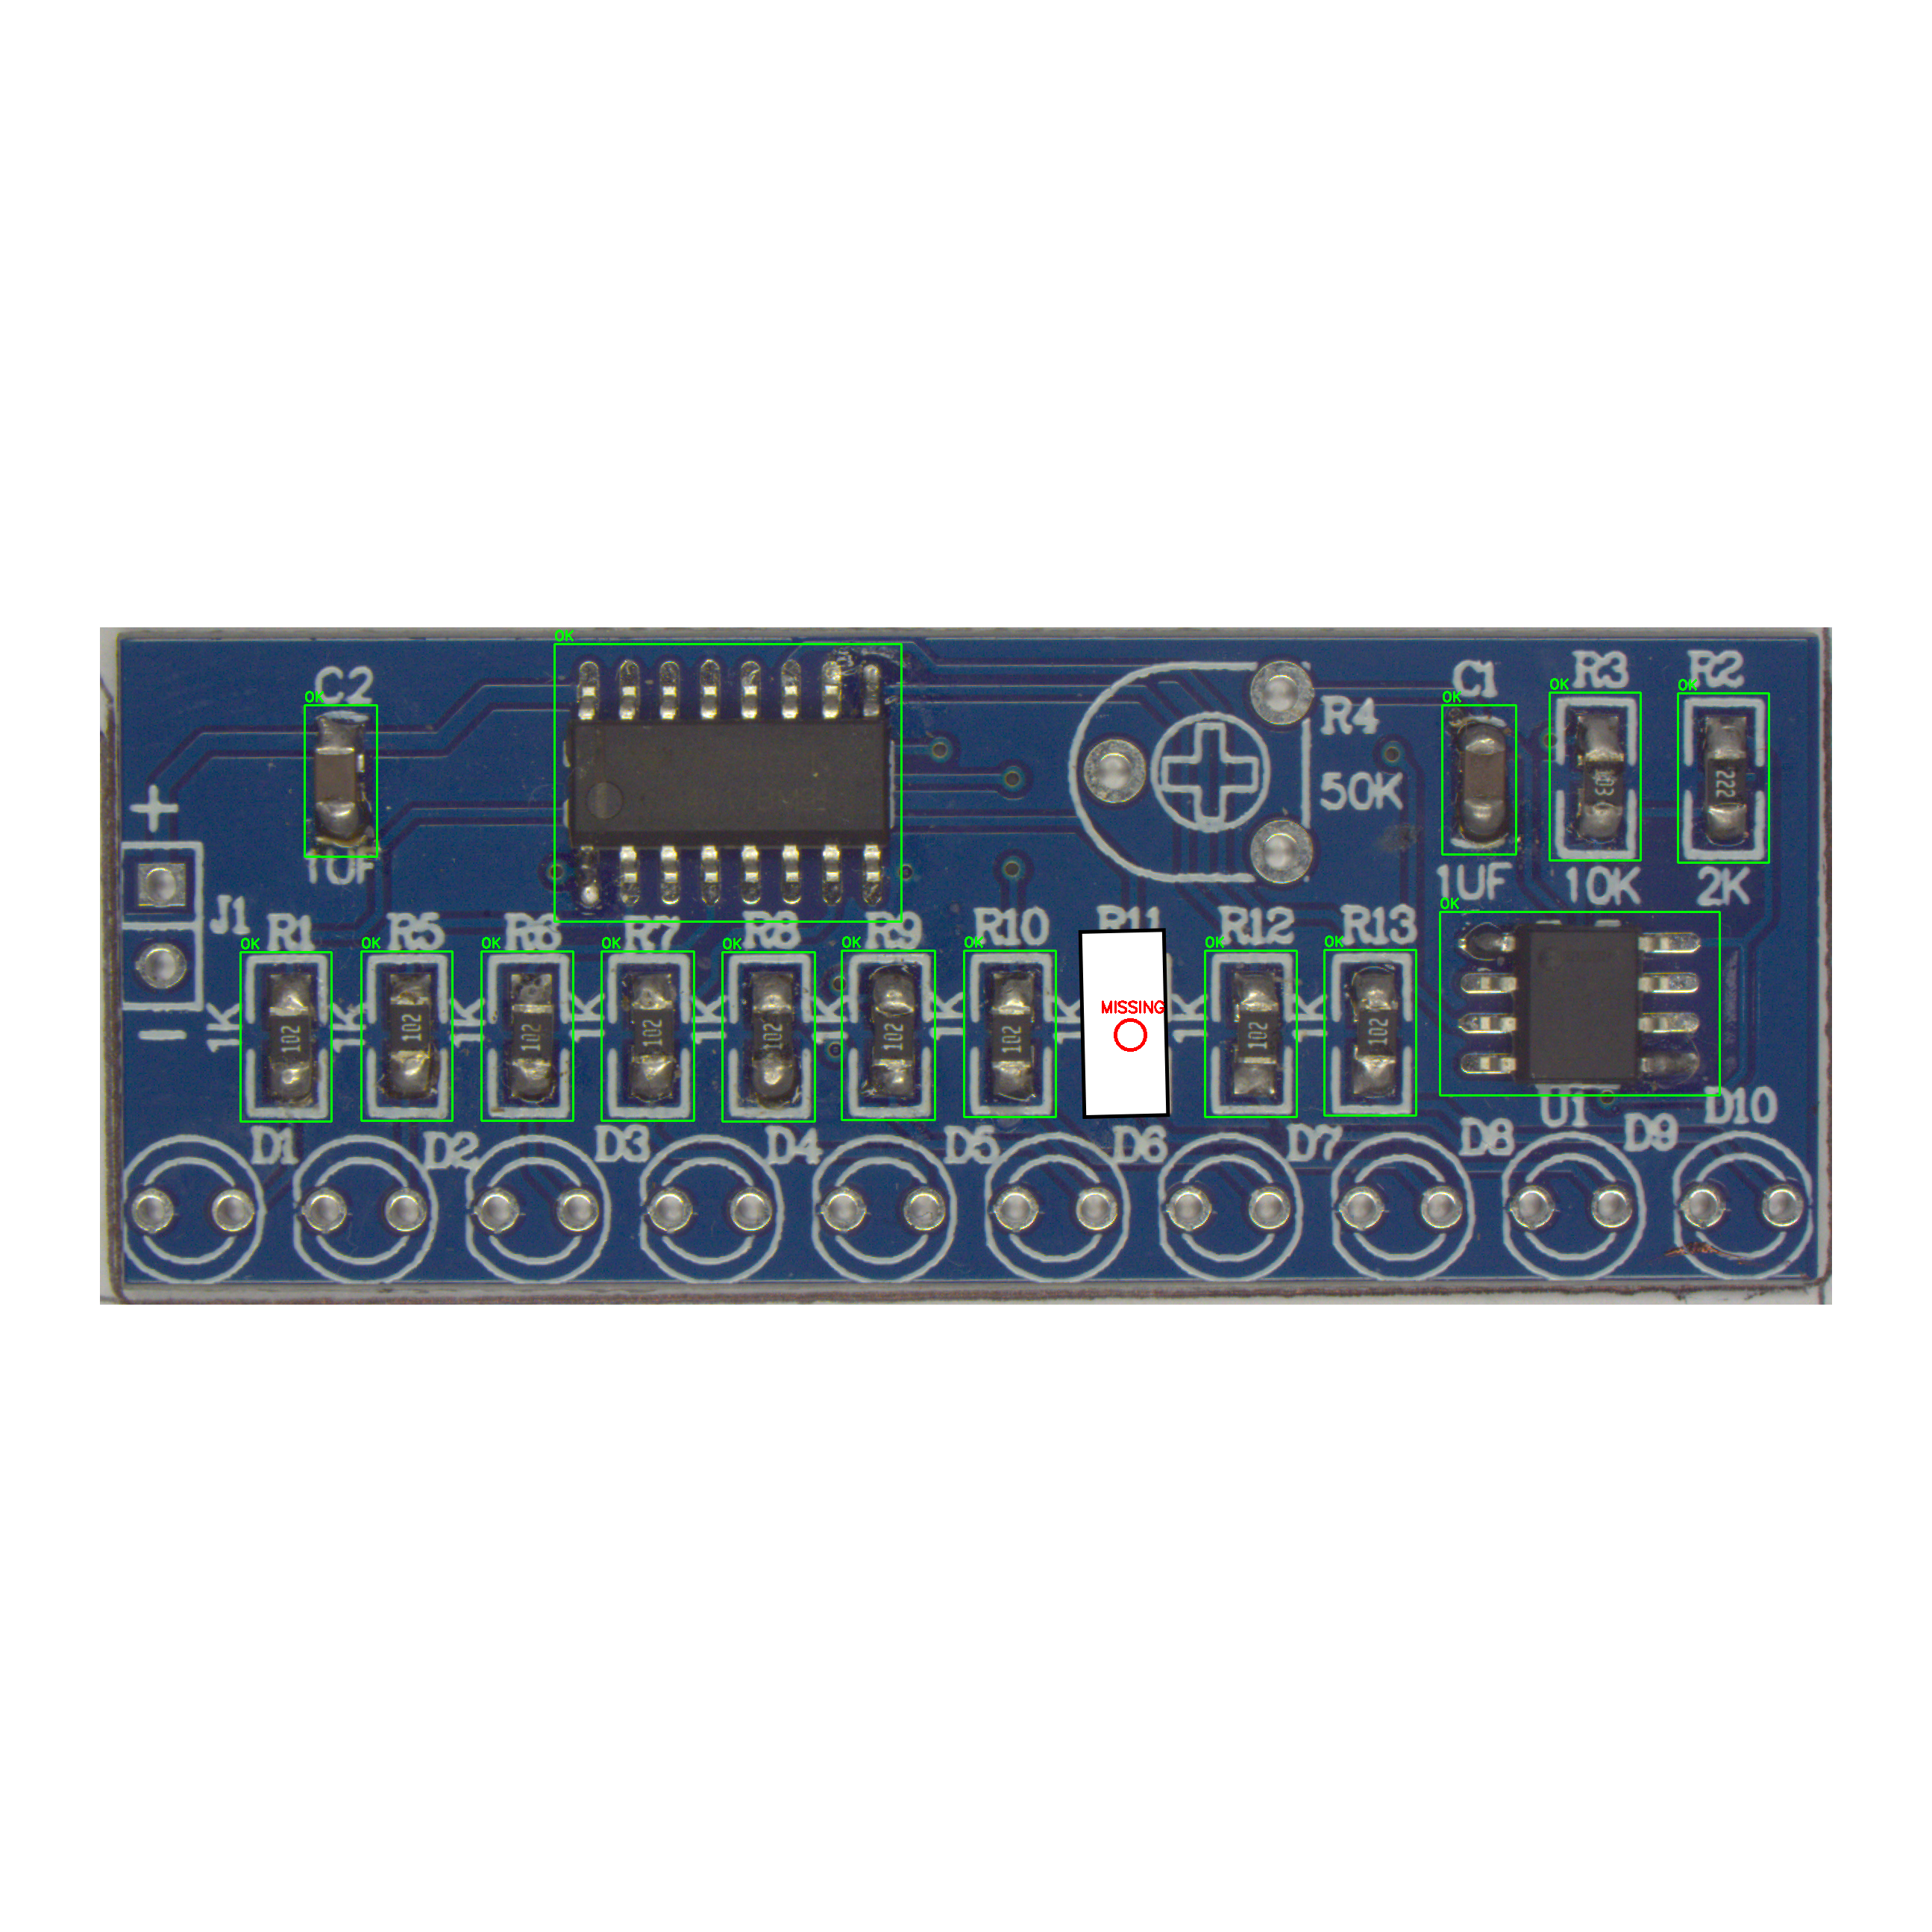
\includegraphics[width=0.48\columnwidth]{defect_missing.png}
    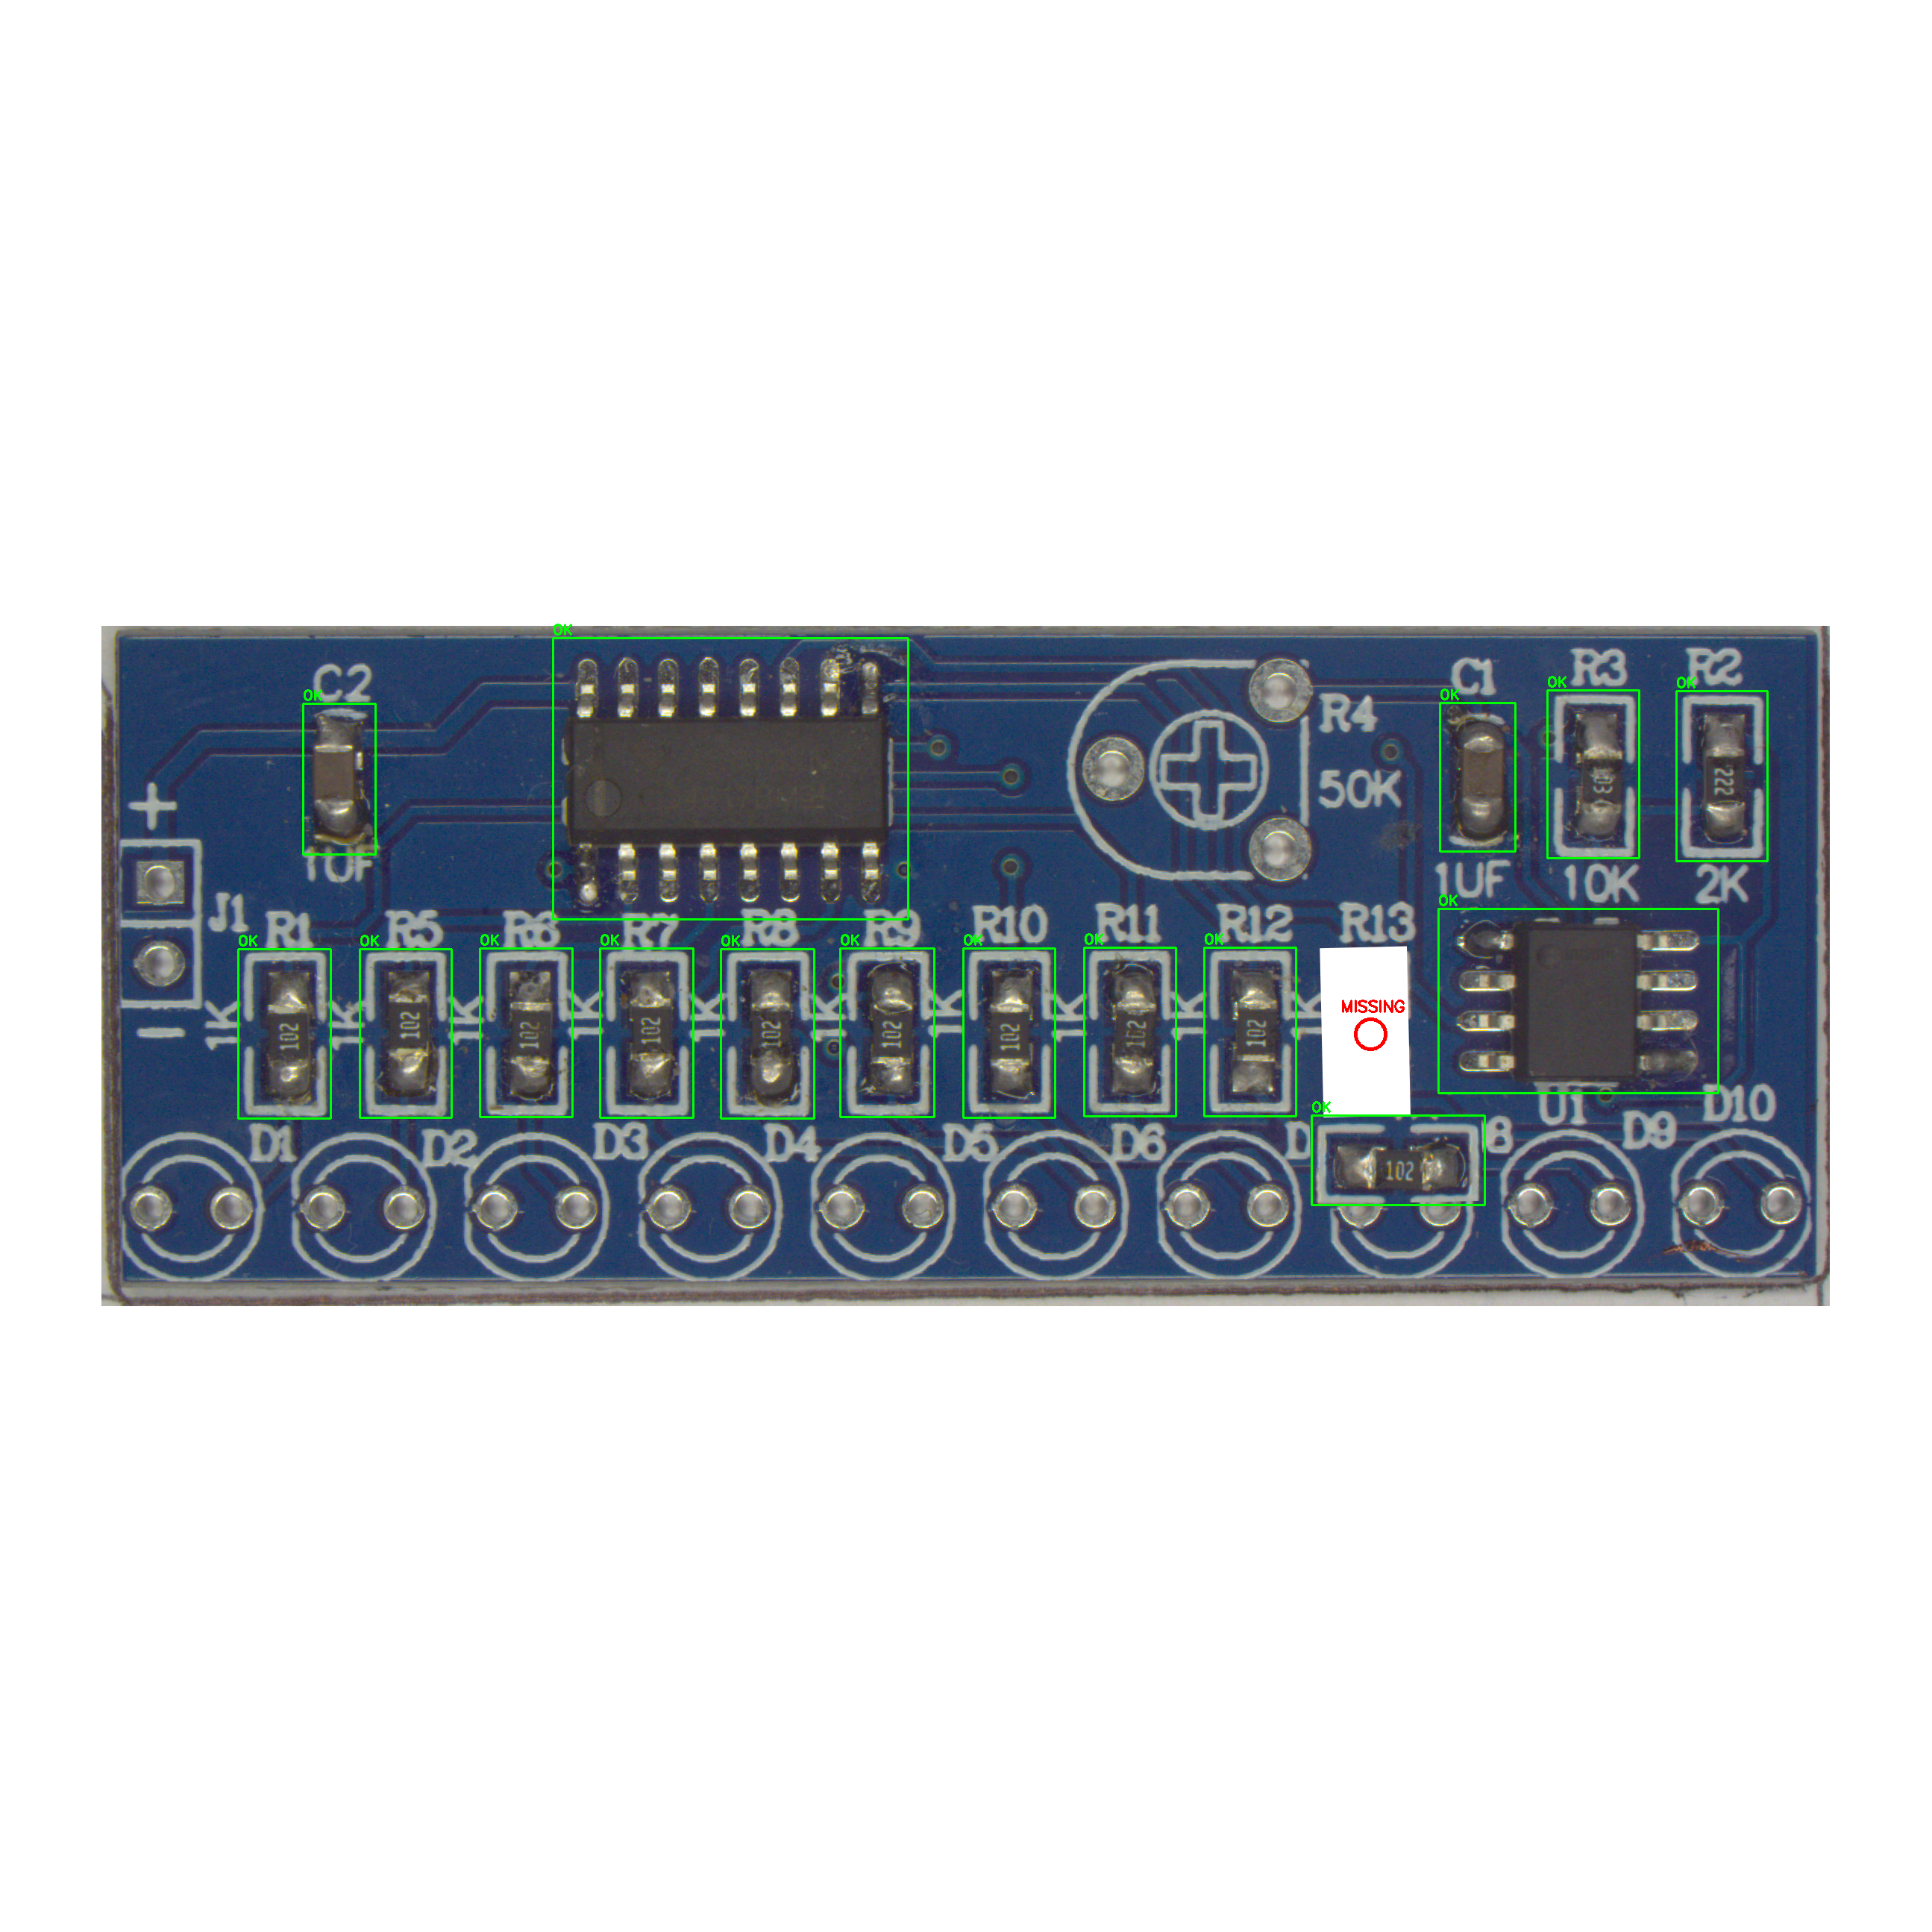
\includegraphics[width=0.48\columnwidth]{defect_shifted.png}
    \caption{Examples of detected defects: missing component (left) and
    shifted component (right). \TODO{replace with side-by-side comparison
    of RGB baseline vs.\ DS-YOLO predictions on the same board}}
    \label{fig:qual_detect}
\end{figure}

\subsection{Discussion and Limitations}
The experiments support all three hypotheses, with the strongest gains
on geometric defect classes and on small training budgets. Two
limitations are worth noting. First, the method assumes that the golden
reference is geometrically registrable to the capture; in practice this
required a controlled fixture and a diffuse dome light, but no specific
hardware beyond what is already present in standard AOI cells. Second,
DS-YOLO inherits the classical limitation of supervised detectors: it
can only flag defect modes that are represented in the training labels.
Combining DS-YOLO with an unsupervised anomaly-detection branch
(e.g.\ PaDiM \TODO{cite}) is a natural direction for future work.

%==============================================================================
\section{Conclusion}
\label{sec:concl}

We have presented Dual-Stream YOLO (DS-YOLO), a Siamese extension of
YOLOv8m that exploits the golden reference image always available in
an AVI cell by routing both the captured frame and the reference
through a shared backbone and fusing their multi-scale features at
$P_3,P_4,P_5$ via a learnable Cross-Reference Fusion Module. The CRFM
adds only $\sim\!70\,$K parameters, preserves the rest of the backbone
and is initialised so the network starts as the YOLOv8m baseline. On a
real SMT production cell that integrates a Mitsubishi PLC, two
articulated robots and an industrial GigE camera through CC-Link and
OPC~UA, DS-YOLO improves mAP@0.5 by
$+\TODO{$\Delta$}$ pp over the RGB-only baseline, with the largest gains
on geometric defect classes and small training budgets, and adds less
than \TODO{$\delta t$}~ms to the per-board latency. Future work will
investigate (i) end-to-end learning of the alignment together with the
detection, (ii) integration of an unsupervised anomaly branch for
unlabeled defect modes and (iii) extension to multi-view six-side
inspection for full board coverage.

%==============================================================================
\section*{Acknowledgment}
\TODO{Acknowledge funding source / lab equipment / etc.}

%==============================================================================
\bibliographystyle{IEEEtran}
\bibliography{refs}

\end{document}
